
c) Para 10 días antes del vencimiento:

%La tabla ira centrada
\begin{center}
 \renewcommand{\arraystretch}{1.5}% Margenes de las celdas
 %Creación de la cuadricula de 3 columnas
\begin{longtable}[H]{|p{0.33\linewidth}|p{0.33\linewidth}|p{0.33\linewidth}|}
	%Creamos una linea horizontal
	\hline
	%Definimos el color de la primera fila
	\rowcolor[HTML]{FFB183}
	%%%%% INICIO ASIGNACIÓN FECHA FOCAL %%%%%%%
	%%%%%%%%%% INICIO TITULO
	%Lo que se hace aquí es mezclar las 3 columnas en una sola
	\multicolumn{3}{|c|}{\cellcolor[HTML]{FFB183}\textbf{1. Asignación período focal}}                   \\ \hline
	%%%%%%%%%% FIN TITULO
	%%%%% INICIO DECLARACIÓN DE VARIABLES %%%%%%%
	\multicolumn{3}{|c|}{$pf :\frac{10}{365} \ = \ 0.027\textit{ pv}$}                                                      \\ \hline
	%%%%%%%%%% INICIO TITULO
	%Lo que se hace aquí es mezclar las 3 columnas en una sola
	\multicolumn{3}{|c|}{\cellcolor[HTML]{FFB183}\textbf{2. Declaración de variables}}                 \\ \hline
	%%%%%%%%%% FIN TITULO
	%%%%%%%%%% INICIO SUBTITULO
	\multicolumn{1}{|c|}{\cellcolor[HTML]{FFB183}\textbf{Valores monetarios}}    & 
	\multicolumn{1}{|c|}{\cellcolor[HTML]{FFB183}\textbf{Valores no monetarios}} &
	\multicolumn{1}{|c|}{\cellcolor[HTML]{FFB183}\textbf{Incógnitas}}  \\ \hline
	%%%%%%%%%% FIN SUBTITULO
	%%%%%%%%%% INICIO DE MATEMÁTICAS
	%Cada & hace referencia al paso de la siguiente columna
 	$F =  100 \ COP$    &  $i_r = 30\%\textit{ pv}  $              & $i_v=? \% \textit{ pv}$  \\                                                                   &$n  = \frac{10}{365} = 0.027\ pv$ & $P_r = ? \  COP$\\
    & $com_v = 0,5\%\textit{ pv}$   &   $P_{v}$  $i_{r}+com_{v}$ \textit{ pv}\\ 
     & & $P_v=?\ COP$ \\
	%%%%%%%%%% FIN DE MATEMÁTICAS
	%%%%% FIN DECLARACIÓN DE VARIABLES
	
	
	%%%%% INICIO FLUJO DE CAJA
	\rowcolor[HTML]{FFB183}
	\multicolumn{3}{|c|}{\cellcolor[HTML]{FFB183}\textbf{3. Diagrama de flujo de caja}}                \\ \hline
	\multicolumn{3}{|c|}{ 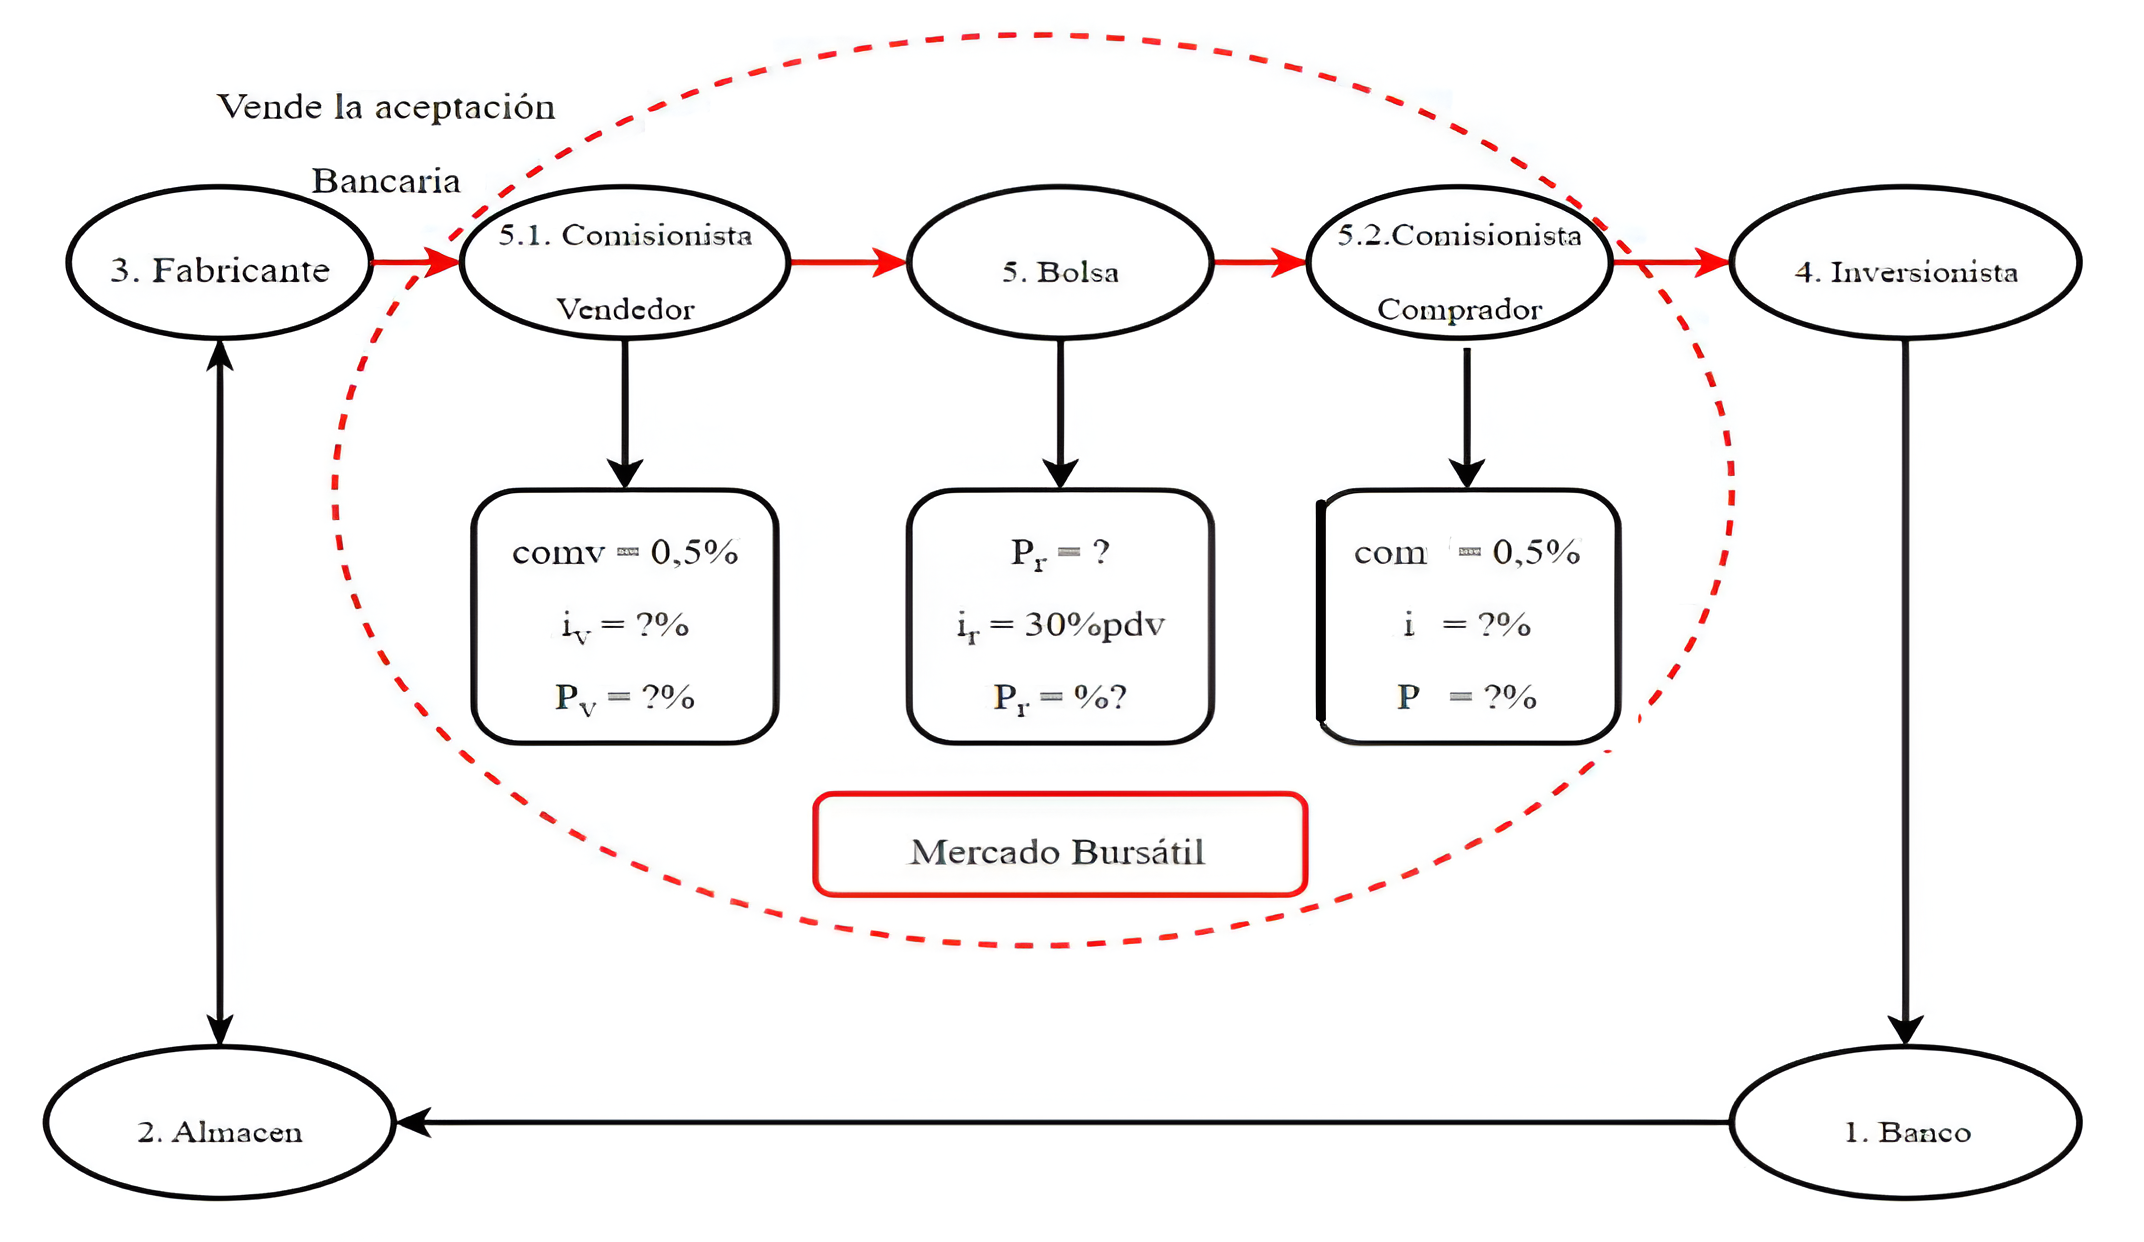
\includegraphics[trim=-5 -5 -5 -5 , scale=0.55, width=16.4 cm, height = 10.5 cm]{3_Capitulo/img/ejemplos/7/7.2c.png} }  \\ \hline
	%%%%%% FIN FLUJO DE CAJA
	
	%%%%% INICIO DECLARACIÓN FORMULAS
	\rowcolor[HTML]{FFB183}
	\multicolumn{3}{|c|}{\cellcolor[HTML]{FFB183}\textbf{4. Declaración de formulas}}                  \\ \hline
	\multicolumn{3}{|C{\textwidth}|}{
		$F = P(1 + i)^n $ \hspace{2mm} Valor futuro 
		
		$I_r$ para calcular $p_r$    
		
		$i_r$ comv para calcular $p_c$
		
		$V_v=? \textit{ COP}$
	}
	\\ \hline
	%%%%% FIn  DECLARACIÓN FORMULAS
	\rowcolor[HTML]{FFB183}
	\multicolumn{3}{|c|}{\cellcolor[HTML]{FFB183}\textbf{5. Desarrollo matemático}}                    \\ \hline
	%Mezclamos 3 columnas y pondremos el dibujo
	%%%%%%%%%%%%% INSERCIÓN DE LA IMAGEN
	%Deberán descargar las imágenes respectivas del drive y pegarlas en la carpeta
	%n_capitulo/img/ejemplos/1/capitulo1ejemplo1.pdf  (el /1/ es el numero del ejemplo)
	\multicolumn{3}{|C{\linewidth}|}{
		
		$P_r =   100 \ COP (1 + 0,30)^\frac{-10}{365} = 99,2838\% \equiv 4{.}964{.}190 \ COP \textit{ Ecuacion de equivalencia}$
		
		$i_v = 0,5\% \hspace{1mm} pv + 30\%\hspace{1mm}pv = 30,5\% \hspace{1mm}pv$
		
		$Pv =  100\ COP(1 + 0, 3050)^\frac{-10}{365}= 99,2733\% \equiv  4{.}963{.}665\ COP $
		
	}                                                                                                  \\ \hline
	
	%%%%% INICIO DECLARACIÓN FORMULAS
	%%%%%%%%%%% INICIO TITULO
	\rowcolor[HTML]{FFB183}
	
	%%%%%% INICIO RESPUESTA
	\rowcolor[HTML]{FFB183}
	%%%%%%%%%%INICIO TITULO
	\multicolumn{3}{|c|}{\cellcolor[HTML]{FFB183}\textbf{6. Respuesta}}                                \\ \hline
	%%%%%%%%%% FIN TITULO
	%%%%%%%%%% INICIO RESPUESTA MATEMÁTICA
	\multicolumn{3}{|C{\textwidth}|}{
		\newline
		$P_r =  4{.}964{.}190\ COP$
		
		$i_v = 30, 5\% \hspace{1mm} pv$
		
		$P_v =  4{.}963{.}665 \ COP$
		
		$P_v = 97,1248\% < p_r = 97,165\% \textit{ COP}$
		\newline
	}                                                                                                  \\ \hline
	%%%%%%%%%% FIN MATEMÁTICAS
	
	
	%%%%%% FIN RESPUESTA
\end{longtable}

 %Se crean dos lineas en blanco para que no quede el siguiente texto tan pegado
 %\newline \newline %USARLO SI CREES QUE ES NECESARIO

\end{center}\

\begin{center}
 \textbf{Tabla resumen para el vendedor}
\end{center}

\begin{center}
\renewcommand{\arraystretch}{2} % Ajusta la altura de la tabla
\setlength{\tabcolsep}{1pt} % Ajusta el espaciado de las columnas
\begin{tabular}{|c|c|c|c|c|c|c|}
\hline
\rowcolor[HTML]{FFB183}
\multirow{2}{*}{} & \multicolumn{3}{|c|}{\textbf{Mercado no bursátil}}  & \multicolumn{3}{|c|}{\textbf{Mercado bursátil}} \\
\cline{2-7}
\rowcolor[HTML]{FFB183}
& \textbf{90 Días} & \textbf{40 Días} & \textbf{10 Días} & \textbf{90 Días} & \textbf{40 Días} & \textbf{10 Días} \\
\cline{1-7}
\textbf{Tasa de registro} & 30\% pv & 30\% pv & 30\% pv & 30\% pv & 30\% pv & 30\% pv \\
\hline
\textbf{Comisión} & 0\% pv & 0\% pv & 0\% pv & 0,5\% pv & 0,5\% pv & 0,5\% pv \\
\hline
\textbf{Tasa R + Com} & 30\% pv & 30\% pv & 30\% pv & 30,5\% pv & 30,5\% pv & 30,5\% pv \\
\hline
\textbf{Precio} & 93,73\% COP & 97,16\% COP & 99,28\% COP & 93,64\% COP & 97,12\% COP & 99,27\% COP \\
\hline
\textbf{Valor de venta} & 4.650.000COP & 4.850.000COP & 4.950.000COP & 4.682.345COP & 4.856.240COP & 4.963.665COP \\
\hline
\end{tabular}
\end{center}

\begin{center}
  \textbf{Conclusiones}
\end{center}
  
\begin{itemize}
  \item Las tasas de registro y comisión son consistentes en ambos mercados para los diferentes períodos de tiempo, lo que facilita la comparación.
  \item En general, los precios y los valores de venta son más altos en el Mercado no bursátil en comparación con el Mercado bursátil para los mismos períodos. Esto puede ser atractivo para el vendedor en busca de mayores ingresos.
  \item Sin embargo, el Mercado bursátil ofrece mayor liquidez, ya que la comisión es ligeramente más alta pero los precios siguen siendo competitivos. Esto puede ser beneficioso si el vendedor necesita vender rápidamente sus activos.
  \item En particular, para el período de 10 días antes del vencimiento, el precio y el valor de venta son más altos en el Mercado no bursátil, lo que puede ser una opción atractiva para maximizar los ingresos en un corto plazo.
  \item En todos los casos, es importante considerar tanto el precio como la liquidez al tomar decisiones sobre la venta de activos financieros en cualquiera de los dos mercados.  \newline
\end{itemize}
  